\section{Procedure}
Goal of the experiment is to adjust an diode laser and measure the absorption spectrum of Rubidium(Rb). 
The first step is to create population inversion inside the laser and take pictures with the help of an IR-Card.
The laser current and the adjustment knobs of the diffraction have to be adjusted until one can observe the laser light.
A sketch of the experimental setup is shown in figure \ref{fig:exp1}.
\begin{figure}
    \centering
    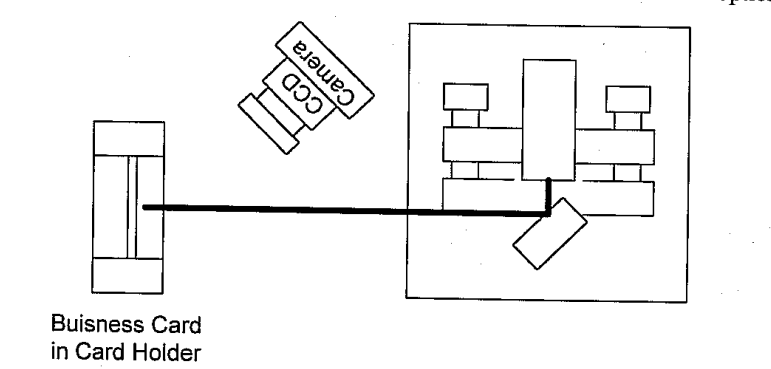
\includegraphics[width = \linewidth]{Bilder/exp1.png}
    \caption{A schematic overview of the experimental setup to observe the population inversion of the laser. Inside the card holder is an IR-Card, which allows one to observe the IR-light of the laser, with the help of the CCD camera.\cite{sample}}
    \label{fig:exp1}
\end{figure}
The second step is to shine the laser through a container filled with Rb gas and observe the subsequent emission of fluorescent light.  The experimental setup can be seen in Figure \ref{fig:exp2}. Again the laser current and the knobs of the diffraction granting can be used to adjust the laser. Furthermore the piezo-current, which varies the angle of the diffraction grating slightly, can be used to scan over some wavelength to find the absorption lines of the Rb.
\begin{figure}
    \centering
    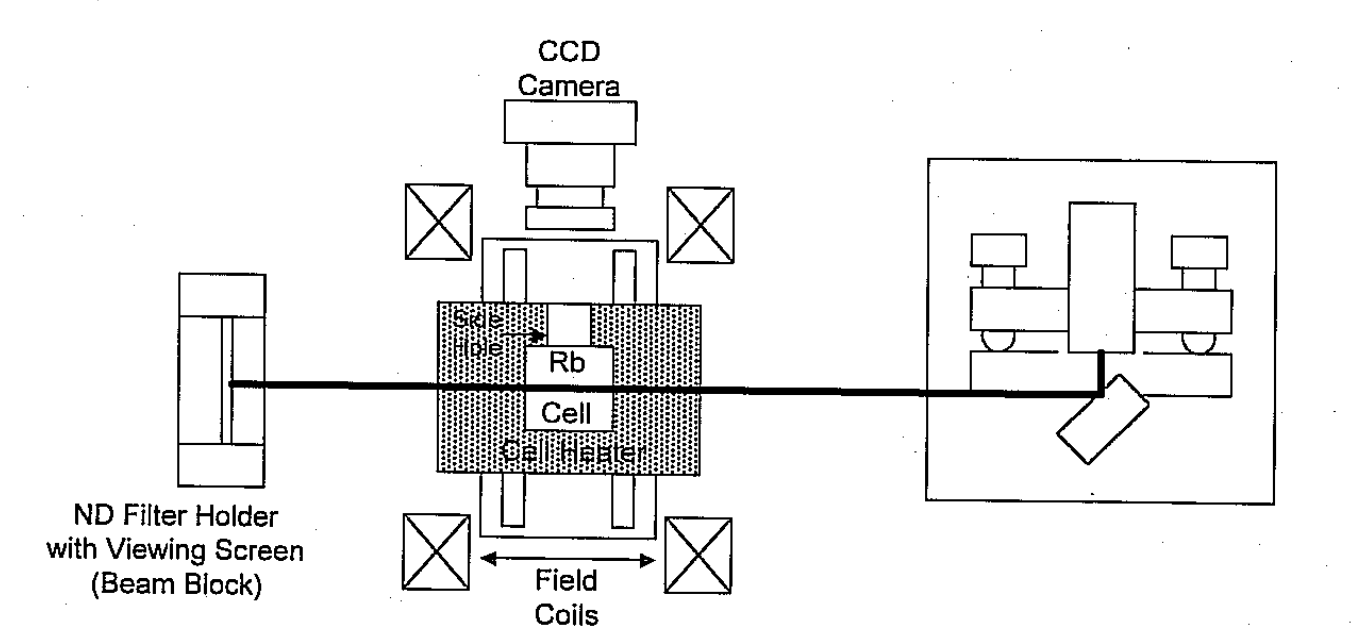
\includegraphics[width = \linewidth]{Bilder/exp2.png}
    \caption{A sketch of the experimental setup, to observe the fluorescent light of the Rb gas. The CCD camera can be used to display the laser and take a photo. }
    \label{fig:exp2}
\end{figure}
To  measure the absorption spectrum, the experimental setup had to be further adjusted. A glass filter and two gelatin filters have to be put between the laser and the Rb cell, which reduces the intensity of the laser beam. 
Furthermore a $50/50$ beam-splitter is installed between the filters and the Rb-cell. The reflected part of the laser beam is adjusted to shine on a photodiode, which is also added to experimental setup. This serves as a measurement of the laser beam, without passing through the Rb gas, and is later used to reconstruct the Rb spectrum.
The transmitted part of the laser beam passes through the Rb cell and shines on another photodiode. The overall setup can be seen in Figure \ref{fig:exp3}.
\begin{figure}
    \centering
    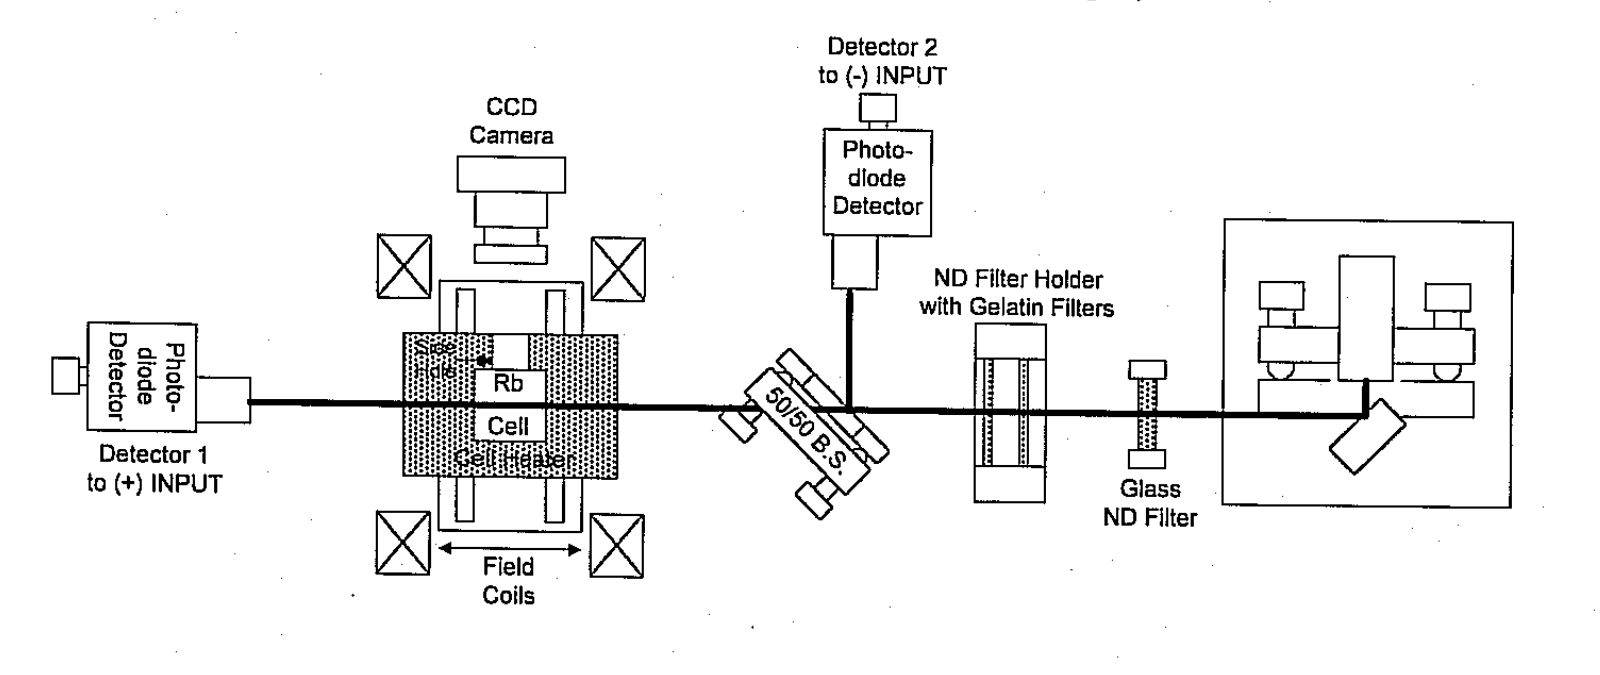
\includegraphics[width = \linewidth]{Bilder/exp3.png}
    \caption{ Overview of the experimental setup for measuring the Rb absorption spectrum. The laser beam is split after passing through several filters and then shines onto two photodiodes, which can be combined to display the spectrum.\cite{sample} }
    \label{fig:exp3}
\end{figure}
The piezo-current is again used to scan over a wavelength region and therefore one is able to display the whole Spectrum and not just a single wavelength.
The two photodiodes get combined by a device, which subtracts out the original laser signal from transmitted light. This allows the display of the Rb spectrum on an oscilloscope. To observe the right spectrum on the oscilloscope, several knobs have to be tuned. This includes the overall gain and the gain of the individual photodiodes.

